\documentclass{article}
\usepackage[T1]{fontenc}
\usepackage[francais]{babel}
\usepackage[utf8]{inputenc}

\usepackage{amsmath,amsfonts,amsthm} % Math packages
\usepackage[pdftex]{graphicx}
\usepackage{hyperref}
\usepackage{lipsum}

\usepackage{listings}
\usepackage{charter}
\usepackage{array}
\usepackage{here}
\usepackage[justification=centering,singlelinecheck=false]{caption}
\usepackage{subcaption}
\newcolumntype{M}[1]{>{\raggedright}m{#1}}
\newcommand{\HRule}{\rule{\linewidth}{0.5mm}}


%Listing Alloy
\lstdefinelanguage{alloy}{
  keywords={%
      assert, pred, all, no, lone, one, some, check, run,
      but, let, implies, not, iff, in, and, or, set, sig, Int, int,
      if, then, else, exactly, disj, fact, fun, module, abstract,
      extends, open, none, univ, iden, seq, enum
  },
  sensitive=true,  % case sensitive
  morecomment=[l]//,%
  morecomment=[l]{--},%
  morecomment=[s]{/*}{*/},%
  morestring=[b]",
  numbers=none,
  firstnumber=1,
  aboveskip=3mm,
  belowskip=3mm,
  frame=single,
  showstringspaces=false,
  numberstyle=\tiny,
  stepnumber=2,
  breaklines=true,
  breakatwhitespace=true,
  tabsize=3,
  basicstyle={\small\ttfamily},
  commentstyle=\itshape,
  columns=flexible,
  keywordstyle=\color{blue}\bfseries,
  ndkeywordstyle=\bfseries,
}

% inline
\def\A{%
    \lstinline[language=alloy,basicstyle=\ttfamily,columns=fixed]}
 
% paragraph
\lstnewenvironment{alloy}[1][]{%
  \lstset{language=alloy,
    floatplacement={tbp},captionpos=b,
    xrightmargin=8pt,basicstyle=\ttfamily,#1}}{}

%Listing Alloy in tab
\lstdefinelanguage{alloyt}{
  keywords={%
      assert, pred, all, no, lone, one, some, check, run,
      but, let, implies, not, iff, in, and, or, set, sig, Int, int,
      if, then, else, exactly, disj, fact, fun, module, abstract,
      extends, open, none, univ, iden, seq, enum
  },
  sensitive=true,  % case sensitive
  morecomment=[l]//,%
  morecomment=[l]{--},%
  morecomment=[s]{/*}{*/},%
  morestring=[b]",
  numbers=none,
  firstnumber=1,
  aboveskip=3mm,
  belowskip=3mm,
  showstringspaces=false,
  numberstyle=\tiny,
  stepnumber=2,
  breaklines=true,
  breakatwhitespace=true,
  tabsize=3,
  basicstyle={\small\ttfamily},
  commentstyle=\itshape,
  columns=flexible,
  keywordstyle=\color{blue}\bfseries,
  ndkeywordstyle=\bfseries,
}

% paragraph
\lstnewenvironment{alloyt}[1][]{%
  \lstset{language=alloyt,
    floatplacement={tbp},captionpos=b,
    xrightmargin=8pt,basicstyle=\ttfamily,#1}}{}
 

 
\usepackage{color}
\definecolor{dkgreen}{rgb}{0,0.6,0}
\definecolor{gray}{rgb}{0.5,0.5,0.5}
\definecolor{mauve}{rgb}{0.58,0,0.82}

\begin{document}

%\title{Génération et analyse automatisées d’ensembles de règles pour Picobot}
%\author{Quentin BAILLEUL \  Jérémy BOSSUT \  Romain PHILIPPON}


%\maketitle
\begin{titlepage}
\begin{center}

% Upper part of the page. The '~' is needed because \\
% only works if a paragraph has started.

\includegraphics[width=0.5\textwidth]{pictures/ul.png}~\\[1cm]

% Title
\HRule \\[0.2cm]
{ \huge \bfseries Génération et analyse automatisées d’ensembles de règles pour Picobot \\[0.4cm] }

\HRule \\[1.5cm]
Quentin BAILLEUL \  Jérémy BOSSUT \  Romain PHILIPPON

\vfill

% Bottom of the page
{\large \today}

\end{center}
\end{titlepage}

\newpage
\tableofcontents

\newpage

\section{Introduction}

Picobot\footnote{\label{pico_lien}\url{https://learn.cs.uml.edu/ext/picobot/}} est un projet utilisé comme support au cours introductoire d'informatique du Dr. Zachary Dodds au Harvey Mudd College de Californie. Ce programme modélise le comportement d’un robot-aspirateur dont le but est d’examiner tous les emplacements inoccupés de son environnement. Il est possible de programmer le robot en lui fournissant un ensemble de règles à respecter.
\\

Notre projet utilise le langage de spécification déclaratif Alloy pour générer ces règles. L'objectif est de chercher le plus petit ensemble de règles qui permet au robot de parcourir l’ensemble d’un niveau, quelque soit sa position initiale.
\\

Nous présentons le fonctionnement du programme Picobot en détails dans la section~\ref{sec:picobot} et les modèles Alloy utilisés dans la section ~\ref{sec:mod_alloy}. Les sections ~\ref{sec:result} et ~\ref{sec:ana_result} montrent respectivement les résultats obtenus et leur analyse. Enfin nous concluons notre travail dans la section ~\ref{sec:conclusion}.


\section{Picobot}
\label{sec:picobot}
Le robot Picobot se trouve dans un environnement rectangulaire modélisé par un tableau de cellules. Les cellules peuvent être inoccupées ou contenir un mur empêchant le passage du robot. Le robot est uniquement capable de percevoir l’occupation des cellules alentours. Comme il n’est pas doté de mémoire interne alors il ne peut pas savoir sur quelle cellule il se trouve et s’il l’a déjà parcourue. Il n’est donc pas possible d’utiliser un algorithme de recherche de chemins tel que Dijkstra ou A*\footnote{\label{pathginding_lien}\url{http://fr.wikipedia.org/wiki/Recherche\_de\_chemin/}}.
\\

Pour se déplacer, le robot respecte un ensemble de règles pré-établies. Une règle est formée de la façon suivante:
\begin{center}
\textit{CurrentState Surroundings} -> \textit{MovementDirection NewState}
\end{center}

\textit{CurrentState} et \textit{NewState} sont deux nombres entiers compris entre 0 et 99. Ces nombres représentent le numéro de l’état dans lequel se trouve le robot respectivement avant et après l’exécution de la règle. Au lancement du programme, le robot se trouve dans l’état 0.
\newpage
\textit{Surroundings} est une chaîne de quatre caractères représentant l’occupation des cellules voisines. Les environnements possibles sont les suivants : 


\begin{figure}[H]
\centerline{
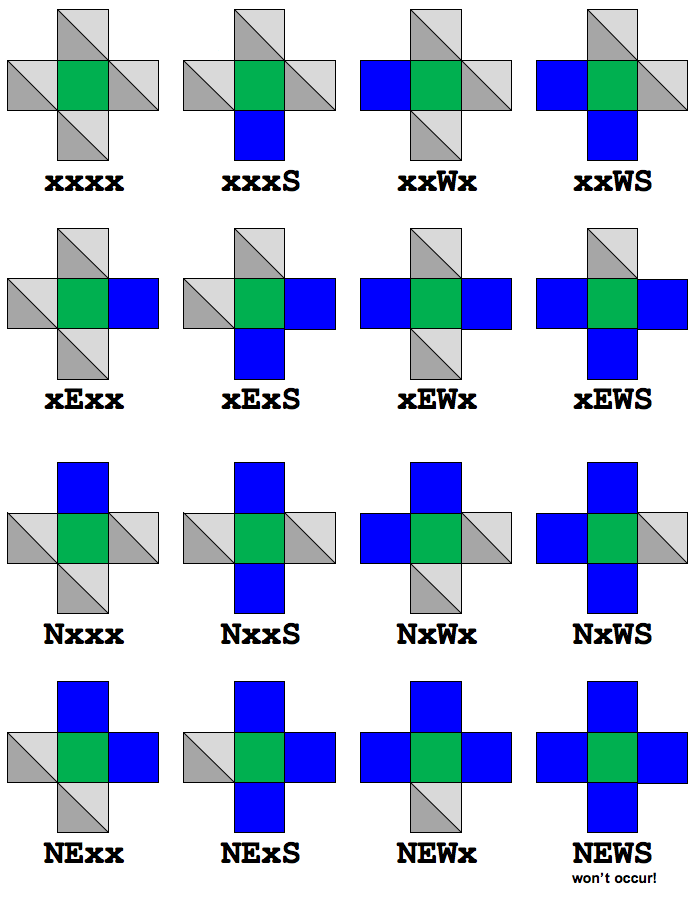
\includegraphics[scale=0.3]{pictures/Image0.png}}
% Legende : 
\caption{Environnements possibles du robot}
\end{figure}

Il est possible de remplacer un des caractères par ‘*’. Le caractère ‘*’ signifie qu’on ne se soucie pas de la présence ou non d’un obstacle à l’emplacement désigné.
\vspace{5mm}

\textit{MovementDirection} représente la direction dans laquelle on souhaite que le robot se déplace. Le robot peut se déplacer dans les quatre directions cardinales (N pour Nord, E pour Est, W pour Ouest, S pour Sud) ou choisir de ne pas bouger (X).
\\\\
\noindent\textbf{Exemple} : Considérons l’ensemble de règles pour Picobot suivant.
\begin{center}
\texttt{0 x*** -> N 0\\
0 N*** -> W 1\\
1 ***x -> S 1\\
1 ***S -> X 0}
\end{center}

\begin{figure}[H]
 \centerline{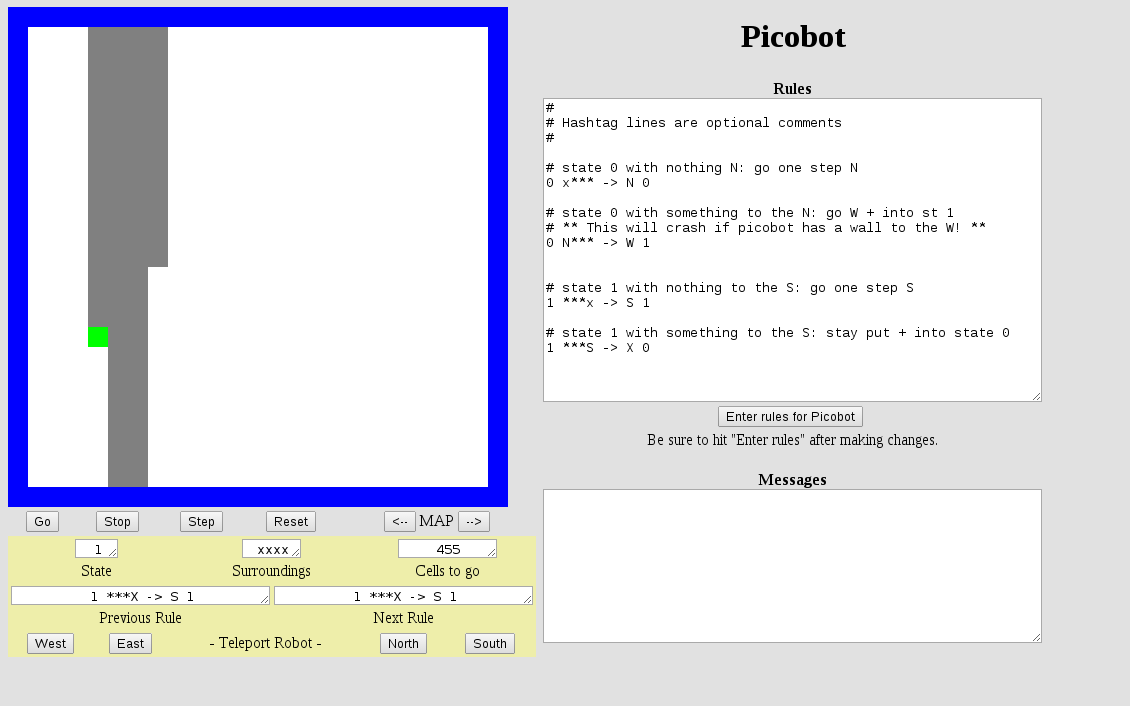
\includegraphics[scale=0.45]{pictures/Image1.png}}
\caption{Représentation du robot Picobot (carré vert) parcourant un niveau en respectant les règles indiquées dans le champ Rules}
 \end{figure}

La règle \texttt{0 x*** -> N 0} est suivie lorsque le robot est dans l'état 0 et qu'il détecte une cellule libre au Nord. Lorsque cette situation se produit, le robot se déplace d'une unité vers le Nord et reste à l'état 0. Lorsque le robot rencontre un obstacle au Nord, la règle \texttt{0 N*** -> W 1} change son état à 1 et le fait se déplacer vers l’Ouest. Une fois le robot dans l'état 1, il suit la règle règle \texttt{1 ***x -> S 1} et va se déplacer vers le Sud jusqu'à ce qu'il rencontre un mur dans cette direction. Dans ce cas, il revient à l'état 0 selon la règle \texttt{1 ***S -> X 0}.

\section{Modèles Alloy}
\label{sec:mod_alloy}
Le caractère ‘*’ a été introduit dans le but d’obtenir une représentation plus succincte des règles. Pour tout ensemble de règles qui utilise ce caractère, il est alors possible de trouver un ensemble de règles équivalent qui ne l’utilise pas.


\begin{figure}[H]
\centering{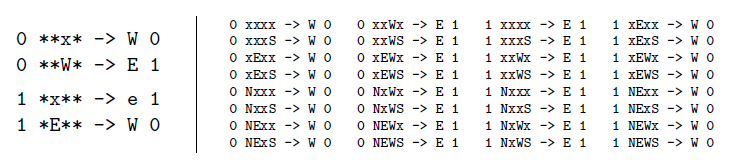
\includegraphics[scale=0.7]{pictures/Image2.png}}
\caption{Équivalence de deux ensembles de règles (version réduite à gauche, version complète à droite)}
\end{figure}


Dans cette section, nous présentons deux modèles Alloy - le premier sans ‘*’ et le second avec - qui permettent de générer des ensembles de règles pour Picobot.

\subsection{Modèle original}
\vspace{5mm}
\begin{figure}[H]
\centerline{
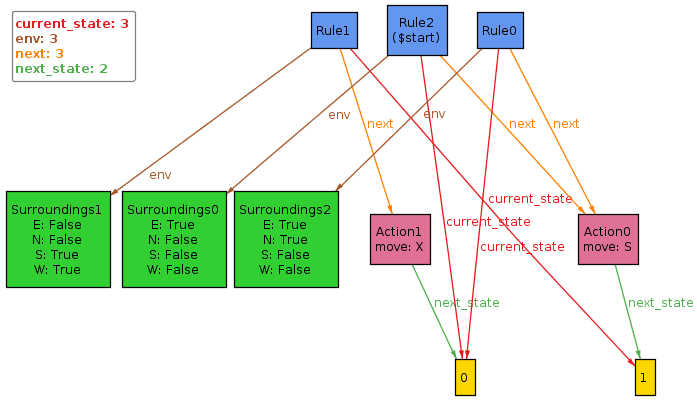
\includegraphics[scale=0.6]{pictures/Image3.png}}
\caption{Représentation schématique d'une instance solution générée par Alloy}
\end{figure}

\newpage
\subsubsection{Ensembles}
Le modèle comprend trois signatures et deux énumérations :
\newline
\begin{figure}[H]
\advance\leftskip-1cm{
\begin{tabular}{|M{5cm}|M{8cm}|}
    \hline
    \textbf{Ensemble} & \textbf{Description} \tabularnewline
    \hline
    \let\centering\relax{
    \begin{alloyt}
sig Rule {
  current_state: Int,
  env: Surroundings,
  next: Action
}\end{alloyt}}& \textbf{Rule} définit une règle applicable où \textit{current\_state} désigne l'état initial du robot, \textit{env} son environnement actuel et \textit{next} l'action à effectuer \tabularnewline
    \hline
    \raggedleft{\begin{alloyt}
sig Surroundings {
  north: Wall,
  east: Wall,
  west: Wall,
  south: Wall 
}\end{alloyt}} & \textbf{Surroundings} définit un environnement en indiquant la présence ou non d'un mur dans chacun des quatre points cardinaux.
\tabularnewline
    \hline
    \centering{\begin{alloyt}
sig Action {
  next_state: Int,
  move: Move
}\end{alloyt}} & \textbf{Action} définit une action à effectuer où \textit{next\_state} désigne le nouvel état du robot et \textit{move} le déplacement à effectuer\tabularnewline
    \hline
    \centering{\begin{alloyt}
enum Move {N, E, W, S, X}
\end{alloyt}} & \textbf{Move} définit les cinq mouvements possibles par le robot: un pour chaque direction cardinale (N,E,W,S) et X pour désigner l’absence de mouvement.
\tabularnewline
    \hline
    \centering{\begin{alloyt}
enum Wall {True, False}
\end{alloyt}} & \textbf{Wall} est identique à l’ensemble des booléens et définit l’état d’un mur (présent: True, absent: False)\tabularnewline
    \hline
 \end{tabular}
}
\end{figure}
\subsubsection{Faits}
Afin de garantir la compatibilité des règles générées avec le programme Picobot, six faits sont utilisés : 


\subsubsection*{Numéro d’état valide}
 Le programme Picobot ne gère que cent numéros d’état numérotés de 0 à 99 :
\newpage
\begin{alloy}
fact validState {
  all r:Rule | r.current_state >= 0 && r.current_state < 100
  all a:Action | a.next_state >= 0 && a.next_state < 100
}
\end{alloy}

\subsubsection*{État initial}
Le robot débutant à l’état 0, il est nécessaire qu'il existe au moins une règle commençant par cet état. De plus, cette règle doit exécuter une action avec un mouvement effectif dans l'une des quatre directions :

\begin{alloy}
fact initialState {
  some r:Rule | r.current_state = 0 && r.next.move != X
}
\end{alloy}

\subsubsection*{Déterminisme du comportement}

Le comportement du robot doit être déterministe. Il ne peut donc pas y avoir d'ambiguïté sur le choix de la règle à appliquer dans une situation donnée. Autrement dit, deux règles ayant le même numéro d'état et le même environnement ne peuvent pas coexister. 

\begin{alloy}
fact noDuplicatedRule {
  all r1: Rule | all r2:Rule-r1 | r1.current_state = r2.current_state => r1.env != r2.env 
}
\end{alloy}

En conséquence, il ne peut pas exister non plus deux instances Surroundings en Alloy qui représente le même environnement.

\begin{alloy}
fact noDuplicatedSurroundings {
  all s1:Surroundings | no s2:Surroundings-s1 | s1.north = s2.north && s1.east = s2.east && s1.west = s2.west && s1.south = s2.south  
}
\end{alloy}

\newpage
\subsubsection*{Enchaînement des règles}
Pour empêcher les règles isolées, il est nécessaire que chaque action emmène vers un état pour lequel il existe une règle.

\begin{alloy}
fact consistentStateNumbers {
  all a:Action | some r:Rule | a.next_state = r.current_state 
}
\end{alloy}
\vspace{5mm}

On s’assure également que chaque action dépend d’une règle pour ne pas avoir d’actions inutilisées qui influent sur le fait précédent.

\begin{alloy}
fact allActionsHaveRule {
  all a:Action | some r:Rule | r.next = a
}
\end{alloy}

\subsubsection{Prédicats d’optimisation}
Quatre prédicats sont ajoutés pour générer un meilleur ensemble de règles. Les modifications induites par ces prédicats ne sont pas nécessaires au bon fonctionnement de Picobot mais permettent d'éviter de générer des règles qui ne peuvent pas être appelées ou qui n'apportent aucune plus-value à l'ensemble.

\subsubsection*{Immobilisme}
Une règle qui conserve l’état et n'exécute pas de mouvement bloquerait le robot dans une boucle infinie. Le prédicat suivant permet d'empêcher la génération de ce type de règles.

\begin{alloy}
pred neverHoldStill {
  all r:Rule | r.next.move = X => r.next.next_state != r.current_state
}
\end{alloy}
\vspace{0.5cm}

Puisque le robot ne peut pas se retrouver dans une situation où il est encerclé de murs, il n'est pas nécessaire de générer un Surroundings où les quatre directions sont bloquantes.
\begin{alloy}
pred neverStucked {
  no s:Surroundings | s.north = True && s.east = True && s.west = True && s.south = True
}
\end{alloy}

\newpage

Il n'est pas pertinent de demander au robot de se déplacer dans une direction lorsque l'on sait au préalable qu'elle contient un mur. 

\begin{alloy}
pred noMoveIntoAWall {
  all r:Rule | r.env.north = True => r.next.move != N
  all r:Rule | r.env.east = True => r.next.move != E
  all r:Rule | r.env.west = True => r.next.move != W
  all r:Rule | r.env.south = True => r.next.move != S
}
\end{alloy}

\subsubsection*{Règles inatteignables}
Pour qu’une règle soit atteignable, il faut que son état initial soit accessible depuis une autre règle. Il faut donc, pour chaque règle dont l’état initial \textit{state} est différent de 0, qu’il existe une règle dont l’état initial est différent de \textit{state} qui exécute une action amenant à l’état \textit{state}. Il est important de noter que cette condition est nécessaire mais pas suffisante. Par exemple, dans un ensemble de trois règles dont les transformations d’état sont \texttt{R1: 0 -> 0, R2: 1->2} et \texttt{R3: 2->1}, le prédicat est respecté mais les règles R2 et R3 sont inatteignables.

\begin{alloy}
pred preventInaccessibleRule {
  all r1:Rule | some r2:Rule | r1.current_state != 0 => r1.current_state != r2.current_state && 2.next.next_state = r1.current_state
}
\end{alloy}

\subsubsection{Autres prédicats}
Le modèle comprend également quelques prédicats dont les apports sont essentiellement cosmétiques. Ceux-ci permettent l'utilisation de numéros d’états consécutifs, d'empêcher la génération de deux actions identiques ou d’environnements non utilisés. Ces prédicats n'ayant pas d'influence sur l'ensemble de règles généré, ils sont inactifs par défaut afin d'améliorer les performances d'Alloy.

\subsection{Modèle alternatif}
Le modèle alternatif autorise l'autorisation du caractère ‘*’ pour décrire un environnement. Pour réaliser cette modification, un troisième état est ajouté dans l’énumération \textit{\textbf{Wall}} :

\begin{alloy}
enum Wall {True, False, Star}
\end{alloy}

La mise en place du caractère ‘*’ impose également la création d'un nouveau fait pour garder l'aspect déterministe des ensembles de règles :

\begin{alloy}
fact compatibleRules {
  all r1: Rule | no r2:Rule-r1 | 
  (r1.current_state = r2.current_state) &&
  (r1.env.north = r2.env.north || r1.env.north = Star || r2.env.north = Star) &&
  (r1.env.east = r2.env.east || r1.env.east = Star || r2.env.east = Star) &&
  (r1.env.west = r2.env.west|| r1.env.west = Star || r2.env.west = Star) &&
  (r1.env.south = r2.env.south || r1.env.south = Star || r2.env.south = Star) 
}
\end{alloy}

\subsection{Comparaison des modèles}
\centerline{
\begin{tabular}{|M{6cm}|M{6cm}|}
    \hline
    \textbf{Modèle original} & \textbf{Modèle alternatif} \tabularnewline
    \hline
    Augmente grandement le nombre de règles nécessaires à la réalisation d'un niveau de Picobot & Permet l'utilisation d'une écriture réduite des règles. \tabularnewline
    \hline
    Limite le nombre d'objets Surroundings possibles à $2^4-1=15$ & Augmente le nombre d'objets Surroundings possibles à $3^4-1=80$
 \tabularnewline
    \hline
    Pour 25 instances d'objets, Alloy réduit le problème à :
159374 variables, dont 4350 primaires et 429710 clauses & Pour 25 instances d’objets, Alloy réduit le problème à :
181326 variables, dont 4450 primaires et 480863 clauses. \tabularnewline
    \hline
    \end{tabular}
}
\vspace{5mm}
\section{Résultats}
\label{sec:result}
Le projet simule le comportement de Picobot sur les niveaux suivants :

\begin{figure}[H]
\centering
\begin{subfigure}{.4\textwidth}
  \centering
  
\includegraphics[width=.4\linewidth]{pictures/ImageMap1.png}
  \caption{Niveau Vide}
\end{subfigure}%
\begin{subfigure}{.4\textwidth}
  \centering
  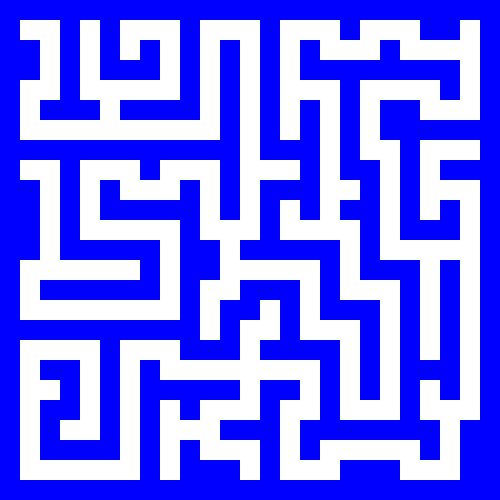
\includegraphics[width=.4\linewidth]{pictures/ImageMap2.png}
  \caption{Niveau labyrinthe}
\end{subfigure}
\caption{Exemples de niveaux}
\end{figure}

Les deux modèles Alloy présentés dans la section précédente sont
testés pour un nombre de 25 instances maximum par objet. Pour des
raisons de performance, le programme se limite à la génération de 500
solutions pour chaque modèle.
\newpage
Nous considérons qu'un ensemble de règles valide un niveau s'il le
complète entièrement quelque soit la position initiale. Chaque
ensemble de règles est alors testé sur toutes les positions inoccupées
dans chacun des deux niveaux.\\

Trois types de résultats sont générés pour chaque ensemble de règles
et pour chaque niveau : le nombre moyen de cases parcourues, la
moyenne du taux de couverture et le nombre de positions initiales qui
permettent à un ensemble de règles de compléter le niveau.

\section{Analyse des résultats}
\label{sec:ana_result}

\subsection{Niveau vide}

Le premier niveau contient 529 espaces inoccupés. A l’exception de 11
ensembles de règles pour le modèle original et 8 pour le modèle
alternatif, tous les ensembles analysés contiennent 4 règles et 2
numéros d’état. Ce faible nombre de règles ne permet pas d’obtenir des
résultats probants.

\subsubsection{Modèle original}

L’ensemble de règles le plus performant permet de parcourir en moyenne
12 des 529 cases. Les 128 ensembles suivants en parcourt entre 9 et
10. De plus, ces ensembles ne permettent de parcourir complètement un
niveau pour aucune des positions initiales possibles.

\subsubsection{Modèle alternatif}

Deux ensembles de règles se distinguent en permettant de parcourir
tout le niveau pour respectivement 42 et 21 positions
initiales. Néanmoins, ces deux ensembles contiennent 25 règles et 4
numéros d’état et le taux de couverture moyen obtenu pour le meilleur
ensemble est de 7,9%.

\newpage
\subsection{Niveau labyrinthe}

Ce niveau, bien que plus complexe, ne contient que 280 espaces
inoccupés. Le modèle alternatif permet de générer un ensemble de
règles qui parcourt tout le niveau dans 82 des 280 points de départ :

\begin{center}
\texttt{3 xxxx -> N 0  \\
3 xEWx -> N 0  \\
3 xxWx -> X 0  \\
3 NxWS -> X 0  \\
3 xExx -> N 0  \\
3 NE*x -> X 1  \\
3 Nx*x -> X 0  \\
3 NxxS -> X 0  \\
3 xExS -> X 2  \\
3 xxxS -> N 0  \\
3 xEWS -> X 0  \\
3 xxWS -> N 0  \\
2 xxWS -> X 0  \\
2 NExx -> X 3  \\
2 Nxxx -> X 3  \\
2 x*Wx -> X 0  \\
1 x*Wx -> X 0  \\
1 xx*S -> X 0  \\
1 *EWS -> X 0  \\
1 Nx*S -> X 0  \\
0 xExS -> N 0  \\
0 NExx -> X 2  \\
0 Nxxx -> X 2  \\
0 x*Wx -> X 1  \\
0 *EWS -> N 0
}
\end{center}

Tous les autres ensembles générés parcourent en moyenne moins de 2
cellules.

\subsection{Remarques}

Bien que permettant la génération d’un nombre plus important
d’environnements différents, le modèle alternatif est plus performant
car il permet une plus grande liberté au robot pour un nombre de
règles équivalent. On peut cependant regretter l’absence de découverte
d’un ensemble de règles qui complète un niveau quelque soit la
position initiale du robot. De plus, la non exhaustivité de l’ensemble
des solutions analysées ne permet pas de s’assurer d’obtenir le
meilleur résultat possible.

\section{Conclusion}
\label{sec:conclusion}
Notre travail montre une preuve de concept de la recherche d’une
solution optimale pour Picobot. Le manque de performance des machines
utilisées n’a néanmoins pas permis d’obtenir une solution
satisfaisante à la problématique posée. Plusieurs pistes
d’amélioration s’ouvrent alors afin de maximiser les performances dont
la simplification du modèle employé ou l’amélioration du filtrage
préalable des ensembles de règles inadaptés. Il serait également
intéressant de poursuivre cette analyse à la recherche d’un ensemble
de règles qui valide plusieurs niveaux.

\end{document}